\documentclass[11pt, a4paper, abstract=true]{scrartcl}
\usepackage[sexy]{evan}
\usepackage{float}
% \usepackage[margin=1in, footskip=14pt]{geometry}
% \clearpairofpagestyles
\setkomafont{pagenumber}{\itshape}
\KOMAoptions{}
\ohead{\footnotesize \textbf{\leftmark}}
\ihead{\footnotesize \textsc{Experiment II}}
\cfoot{\pagemark}

\newcommand{\ve}[1]{\vec{\mathbf{#1}}}
\newcommand{\dt}[1]{\frac{d#1}{dt}}

\begin{document}
\subject{
    PH1102: Experiment II
}
\title{
    \Huge Verification of \\
    Newton's 2nd Law of Motion
}
\author{
    Abhisruta Maity \\
    {\normalsize 21MS006}
    \plusemail{am21ms006@iiserkol.ac.in}
}
\date{}
\publishers{
    \normalsize \emph{Indian Institute of Science Education and Research, Kolkata \\
    Mohanpur, West Bengal, 741246, India}
}
\maketitle
\begin{abstract}
    \sffamily
    In this Experiment II, we tried to verify Newton's 2nd Law of Motion by analyzing a the motion of a moving object with motion-detecting camera and VideoCom software and some computation.
\end{abstract}

\vspace{-2em}

\tableofcontents

\newpage
\section{Theory}
In this experiment, we are going to verify Newton's 2nd Law of motion. The theory that works behind-the-scene of this experiment is discussed in following sections.
\subsection{A Brief History}
From a long time ago, greek philosophers were trying to find some law that relates the cause and effect behind motion of a body. Aristotle (384 BC – 322 BC) proposed that, \emph{the cause} \(F\) of motion of a body is directly proportional to the speed of the body \(v\), i.e, \[F \propto v\] Note that, according to many accepted sources, the notion of vectors were absent in those era.

But people observed that, in some cases, we can push an object (cause of the motion \(F \neq 0\)) but although speed remains zero (\(v = 0\), which we now know as due to an opposing push \emph{static friction} on the object). In contrast, staring some other cases, they noticed \(v \neq 0\) while \(F = 0\) (which is now known as \emph{uniform motion} of a body). It was very intriguing and irritating that time for philosophers to accept.

After a long period, famous philosopher, mathematician Galileo Galilei (1564 – 1642), by analysing moving objects, concluded some \emph{transformation laws} between moving frame of references\footnote{This is the time when first the notion of \emph{Frame of Reference} was introduced.}.

In succeeding, a brilliant philosopher, mathematician Sir Issac Newton re-cited the papers by Galileo and obtained brand-new, precise, consistent and very dynamic law which he presented in his treatise \emph{Philosophae Naturalis Principia Mathematica}. It was indeed a beautiful and clever correction to Aristotle's law of motion . And the concept of vectors elucidated some complex calculations.

\subsection{The Laws}
\begin{definition}[\vocab{Force \(\ve{F}\)}]
    It is a mathematical vector quantity which is interpreted as the cause of motion of a body. It can be felt by our senses.
\end{definition}
\begin{definition}[\vocab{Position \(\ve{x}\)}]
    It is a vector which locates the the object after fixing a frame of reference. It's tail starts from the origin of the frame and ends at the location of the pojnt object.
\end{definition}
\begin{definition}[\vocab{Velocity \(\ve{v}\)}]
    It is a vector which measures `speed' of an object with it's direction of motion. Mathematically, \[\ve{v} \defeq \dt{\ve{x}}\]
\end{definition}
\begin{definition}[\vocab{Acceleration \(\ve{a}\)}]
    It is a vector with measures the rate of change of velocity woith respect to time, i.e., \[\ve{a} \defeq \dt{\ve{v}}\]
\end{definition}
\begin{definition}[Momentum \(\ve{p}\)]
    It is a vector that measures both the \emph{restness} and \emph{movingness}. Mathematically, \[\ve{p} = m\ve{v}\]
\end{definition}
Now we are ready to state the laws of motion of Newton.
\begin{theorem}[Newton's Laws of Motion]
    The three laws are stated as follows\footnote{We are considering only point objects.}:
    \begin{itemize}
        \item If we are observing the motion of an object from an inertial frame, then \[\ve{F} = 0 \iff \dt{\ve{p}} = 0\] Note that, \(\ve{F}\) is here the net force on the object.
        \item In an inertial frame of reference, the net force on an object is proportional to the rate of change of momentum of the body, i.e., \[\ve{F} \propto \dt{\ve{p}}\]
        \item Force exerted by body 1 on body 2 (\(\ve{F'}\)) is exactly equal in magnitude and opposite to the force exerted by body 2 on body 1 (\(\ve{F}\)), i.e., \[\ve{F'} = -\ve{F}\] And both the vectors are lying on the same line joining the centers of two bodies.
    \end{itemize}
\end{theorem}
\begin{remark}
    Our expeiment is on verifying Newton's 2nd law for constant mass. Note that,
    \begin{align*}
        \ve{F} &\propto \dt{\ve{p}} \\ \implies \ve{F} &\propto m\dt{\ve{v}} \\ \implies \ve{F} &\propto m\ve{a} \\ \implies \ve{F} &= km\ve{a}
    \end{align*}
    for some proportionality factor k.
    Now we set the standard unit of mass in such a way that for \(\abs{\ve{a}} = 1 \, \text{m s}^{-2}\) and \(m = 1\) kg, \(\abs{\ve{F}}\) becomes \(1 \, \text{kg m s}^{-2} \defeq 1\) N. Hence, \(k = 1\). In particular we have the well-known equation
    \begin{equation}
        \ve{F} = m\ve{a}
        \label{eq:eq1}
    \end{equation}
    We will experimentally verify Equation \ref{eq:eq1}.
\end{remark}

\subsection{Reverting to 1D motion }
For our practical purposes we remove the vector form of the law by setting up for 1-dimensional motion in laboratory and selecting a proper coordinate frame. We now have 
\begin{equation}
    F = ma
    \label{eq:eq2}
\end{equation} where the meaning of the terms remains as usual.

This was the theoretical behind-the-scene of our experiment. We will now explore the experimental set-up and further deductions.

\section{Experimental Set-Up}
\subsection{Set-up}
A vertically hanging weight (\(m\); can be varied) is connected to a horizontal, almost friction-less (by air-track set-up) slider (can be a cart also), which carries mass (\(M\); can be varied) using pulley-string set-up.
\subsection{Procedure}
We skip this part as instructed in last experiment.
\subsection{Working Formula}
Suppose \(T\) be the \emph{tensile force} of the connecting string. And \(\mu\) be the \emph{coefficient of kinetic friction} For the vertical motion of the hanging mass:
\begin{equation}
    mg - T = ma
    \label{eq:eq3} 
\end{equation}
And for the horizontal movement of the slide on air-track:
\begin{equation}
    T - \mu N = Ma
    \label{eq:eq4}
\end{equation}
where reaction force by the track on the slider is \(N\) and \(N - Mg = 0\) since there is no vertical acceleration of it. Thus
\begin{equation}
    T - \mu Mg = Ma
    \label{eq:eq5} 
\end{equation}
Solving Equation \ref{eq:eq3} and \ref{eq:eq5} we obtain \begin{equation}
    a = \frac{m - \mu M}{m + M} g
\end{equation}
For air-track, we assume \(\mu \approx 0\). Then our equation becomes,
\begin{equation}
    a = \frac{m}{m + M} g
\end{equation}
This is our working formula for this experiment.

\subsection{Flow of the Experiment}
We first observe \(F = mg\) to be net external force on the \(m+M\) system. And for the slider the acting force on it which makes it move is the tension \(T = \frac{2mM}{m + M} g\).
\begin{itemize}
    \item First we keep total mass \(M+m\) to be constant. And then manipulate data and plot \(F\) vs. \(a\) curve. The curve should be somewhat linear after linear regression. And the slope will denote the total mass \(M+m\).
    \item In the other case, we keep \(F\) constant, i.e., the hanging mass \(m\) constant, while varying the mass of the extra mass on the slider \(M (M_s+m_s)\). And then manipulate data and plot \(M\) vs. \(a^{-1}\) curve. In the same way, the slope is expected to denote the net force on the system \(F\).
\end{itemize}
In the next section, we are going to explore all these database anaysis.
\newpage
\section{Data Analysis}
\subsection{Case I: Fixed Total Mass}
First we analyse the position of the slider against time by the camera setup.
\begin{figure}[h]
    \centering
    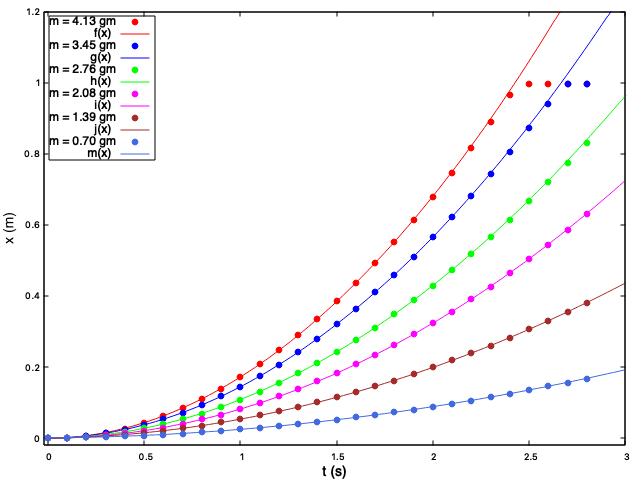
\includegraphics[scale=0.65]{assets/xt_fixed_mass.png}
    \caption{\(x\) vs. \(t\) and non-linear regression through those points}
    \label{fig:fig1}
\end{figure}
We assume 6 different functions \(f(x), g(x), h(x), i(x), j(x)\) and \(m(x)\) for those 6 different set of points such that 
\begin{algorithm}
    \begin{align*}
        f(x) &= c1 + v1 * x + 0.5 * a1 * x^2 \\
        g(x) &= c2 + v2 * x + 0.5 * a2 * x^2 \\
        h(x) &= c3 + v3 * x + 0.5 * a3 * x^2 \\
        i(x) &= c4 + v4 * x + 0.5 * a4 * x^2 \\
        j(x) &= c5 + v5 * x + 0.5 * a5 * x^2 \\
        m(x) &= c6 + v6 * x + 0.5 * a6 * x^2
    \end{align*}
    where \(x\) denotes the the time \(t\) and the corresponding functions denote the positions (or displacement; same here) of the slider.
\end{algorithm}
We have the output of \texttt{GNUPlot} for each regression.

\newpage

\begin{figure}[H]
    \centering
    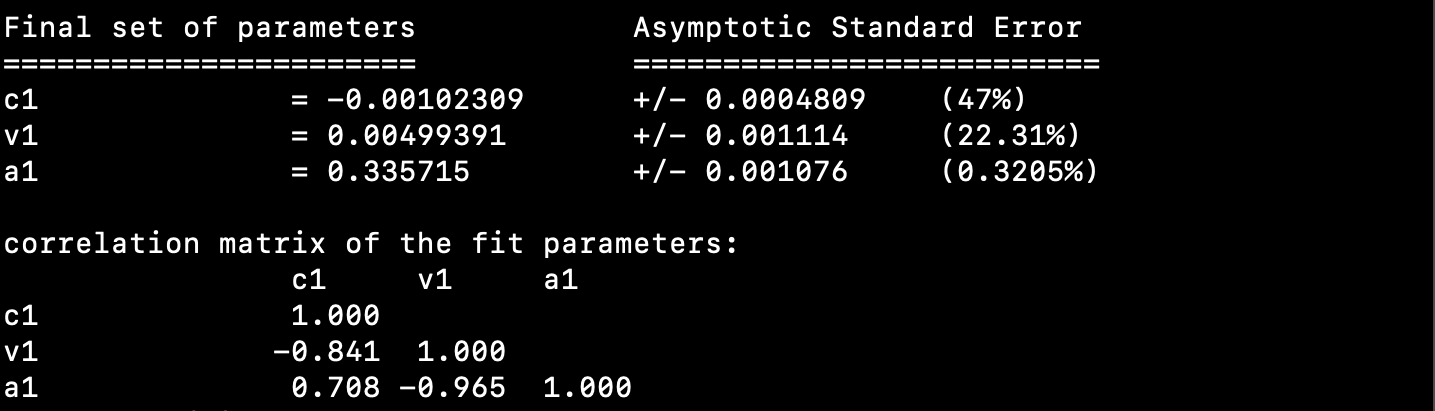
\includegraphics[scale=0.55]{assets/gnuplot_shots/1.png}
    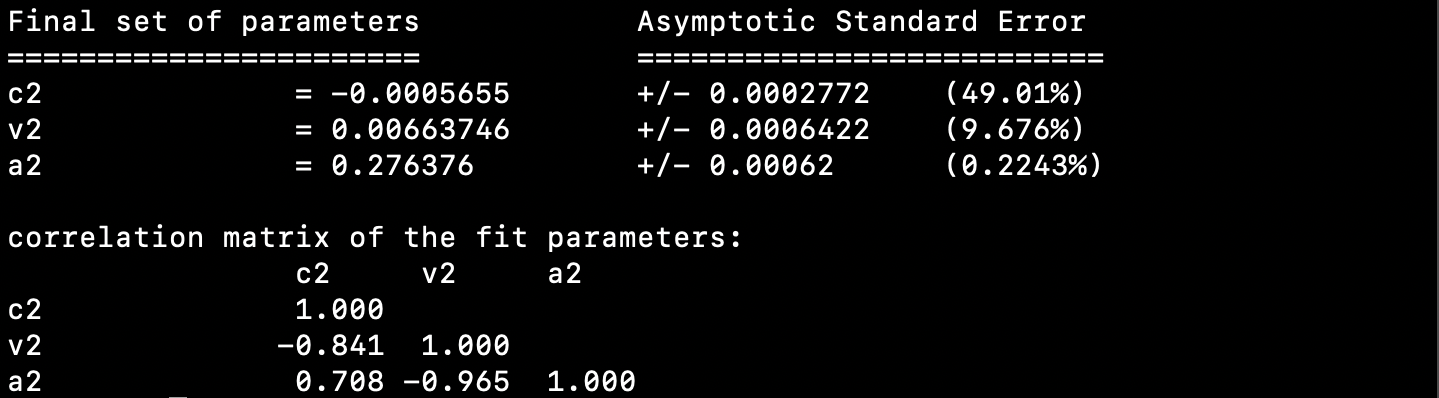
\includegraphics[scale=0.55]{assets/gnuplot_shots/2.png}
    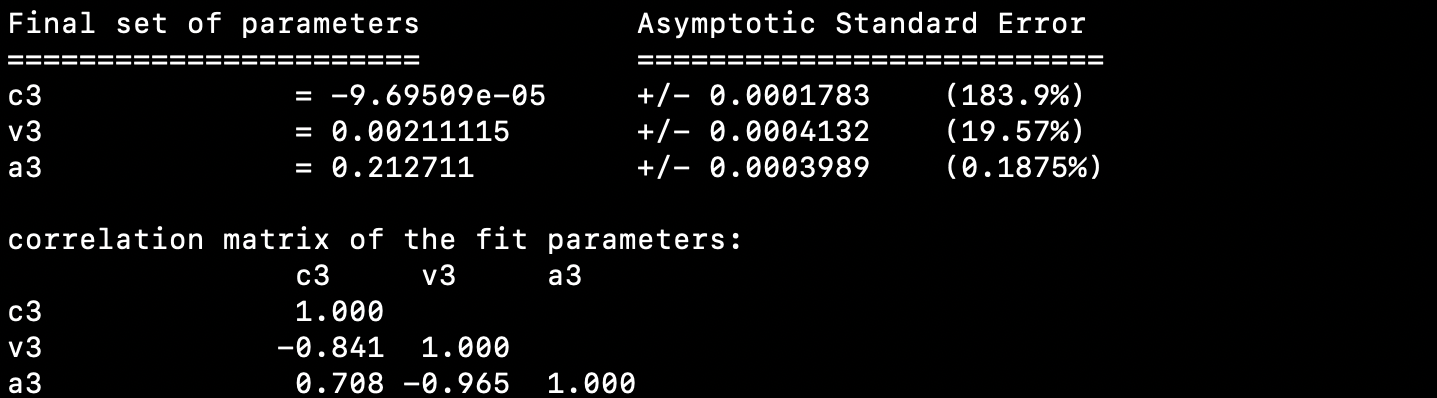
\includegraphics[scale=0.55]{assets/gnuplot_shots/3.png}
    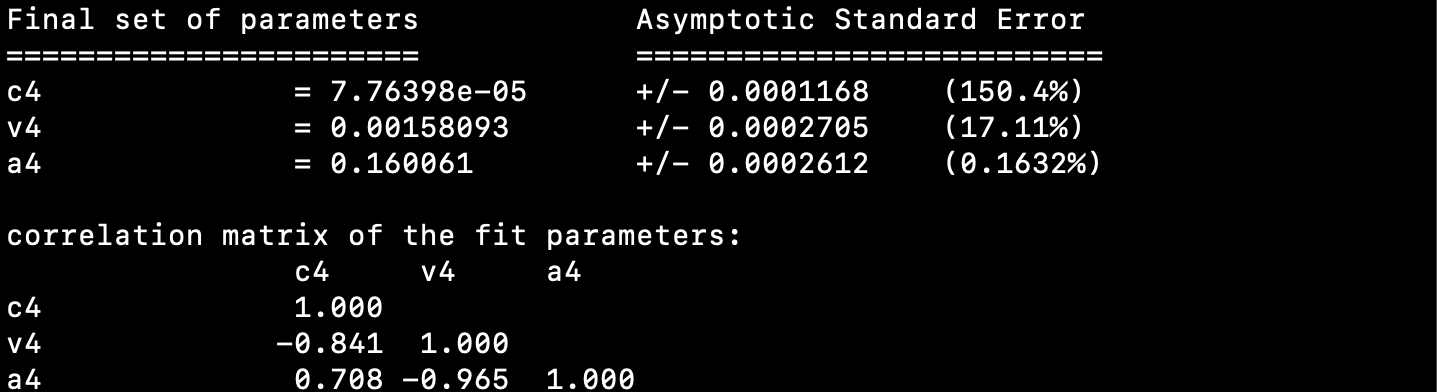
\includegraphics[scale=0.55]{assets/gnuplot_shots/4.png}
    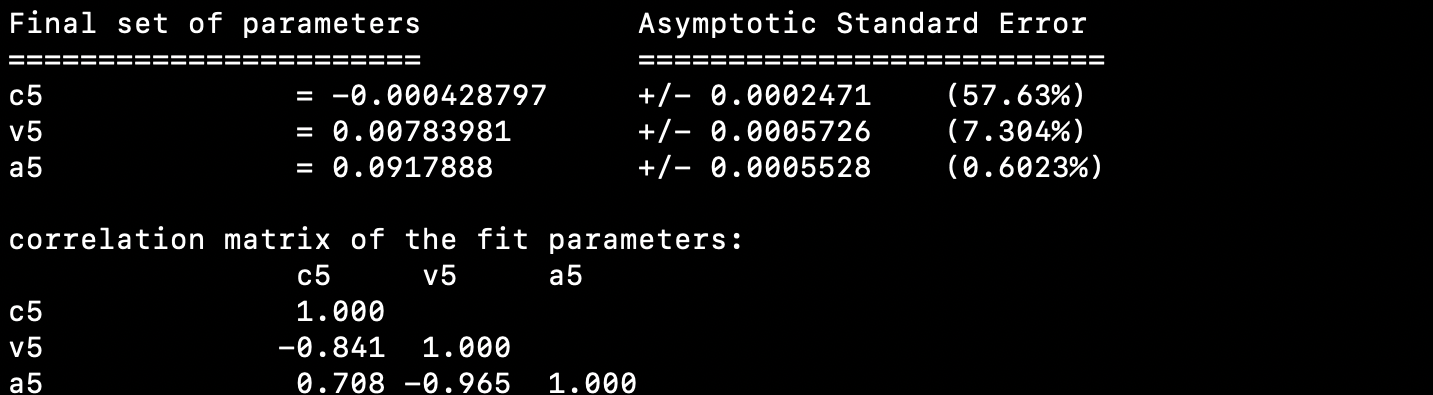
\includegraphics[scale=0.55]{assets/gnuplot_shots/5.png}
    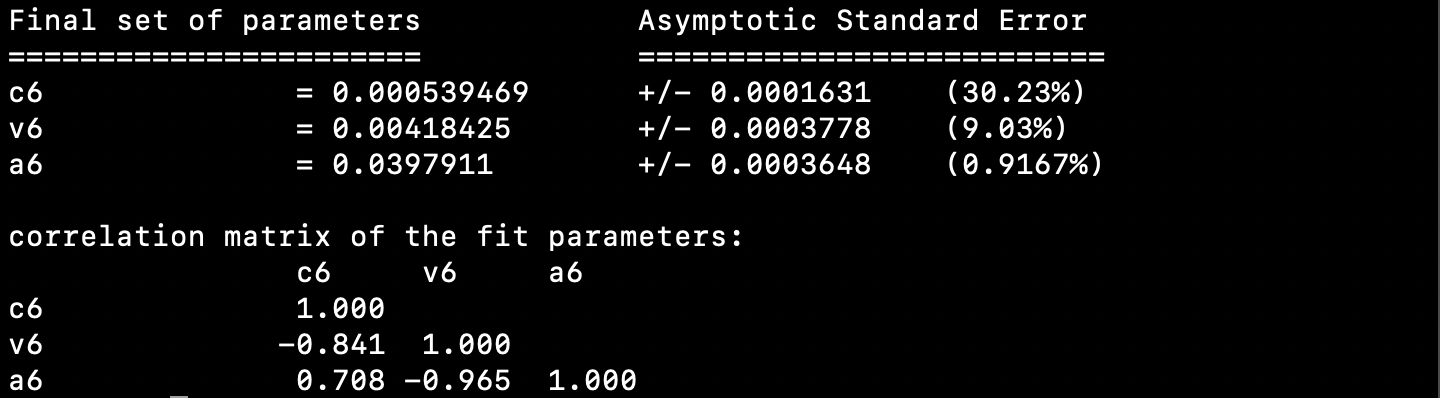
\includegraphics[scale=0.55]{assets/gnuplot_shots/6.png}
    \caption{\texttt{GNUPlot} outputs for the fitting}
    \label{fig:fig2}
\end{figure}

\newpage

Now we plot the corresponding velocity \(v\) and acceleration \(a\) against \(t\).
\begin{figure}[H]
    \centering
    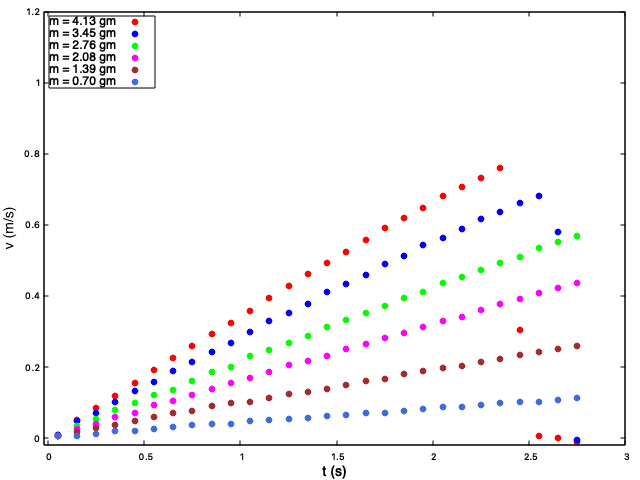
\includegraphics[scale=0.60]{assets/vt_fixed_mass.png}
    \caption{Velocity \(v\) against Time \(t\)}
\end{figure}
\begin{figure}[H]
    \centering
    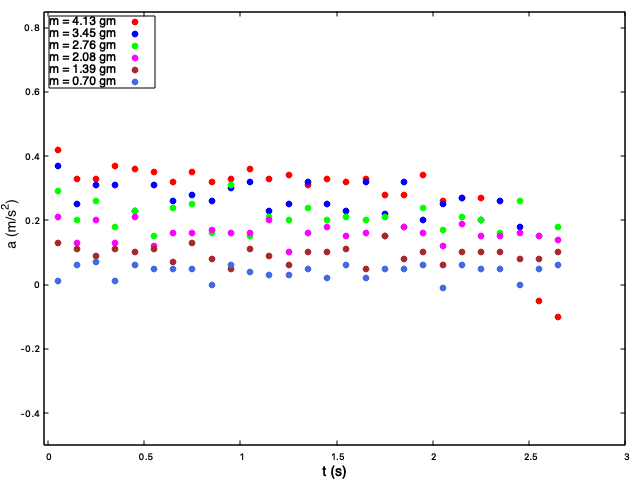
\includegraphics[scale=0.60]{assets/at_fixed_mass.png}
    \caption{Acceleration \(a\) against Time \(t\)}
\end{figure}

\newpage

Now we collect the acceleration values from Figure \ref{fig:fig1} and \ref{fig:fig2} and do a plot of applied force \(F\) against the acceleration \(a\). Then we linearly fit it with a line, whose slope is expected to denote the total mass of the system.
\begin{figure}[H]
    \centering
    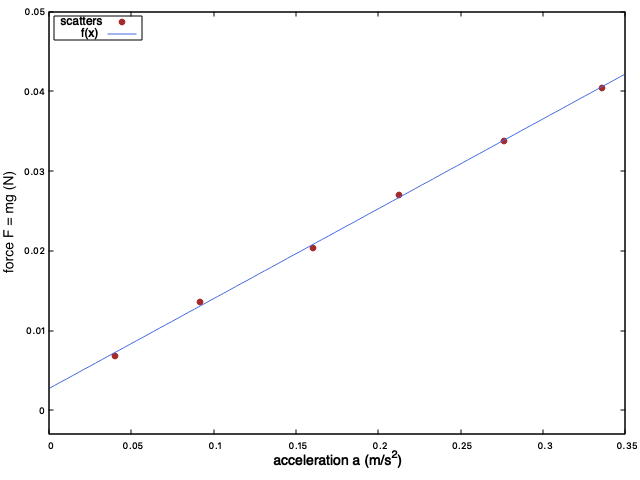
\includegraphics[scale=0.65]{assets/fixedmass_fit.png}
    \caption{The linear fit of \(F\) vs. \(a\)}
\end{figure}
\begin{algorithm}
    We assume the function of regression to be \[f(x) = mx + c\] where \(f(x)\) denotes the Force \(F\) and x being the acceleration \(a\).
\end{algorithm}
And the corresponding \texttt{GNUPlot} window is
\begin{figure}[H]
    \centering
    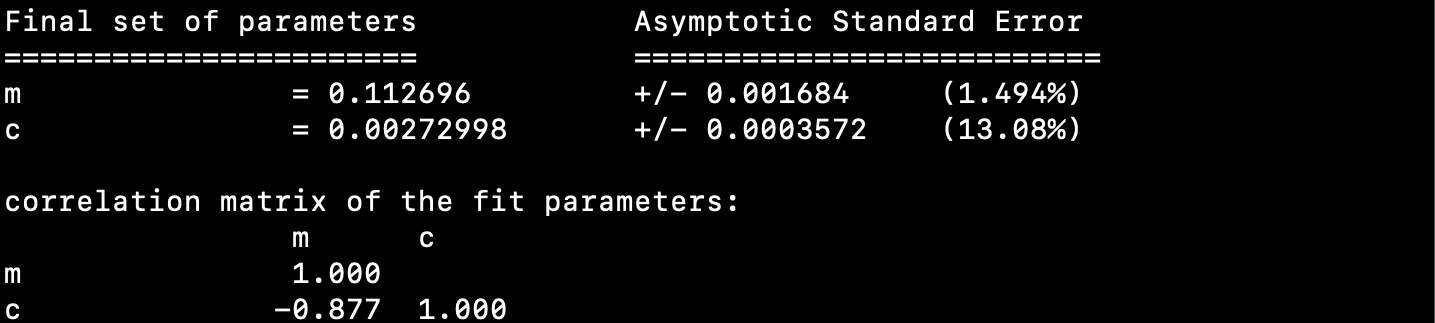
\includegraphics[scale=0.55]{assets/gnuplot_shots/fit.png}
    \caption{\texttt{GNUPlot} window for the linear regression of \(F\) vs. \(a\)}
\end{figure}

\newpage

\subsection{Case II: Fixed Net Force}
As we have done in Case I, again we first analyse the position of the slider against time by the camera setup. As per the database given, we assume 4 different functions \(f(x), g(x), h(x)\) and \(i(x)\) fot the non-linear regression of \(x\) vs. \(t\) such that
\begin{figure}[h]
    \centering
    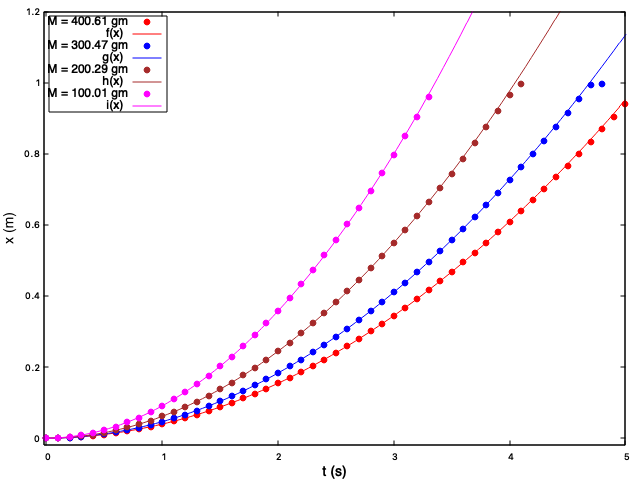
\includegraphics[scale=0.65]{assets/xt_fixed_force.png}
    \caption{\(x\) vs. \(t\) and it's non-linear regression to find acceleration}
    \label{fig:fig7}
\end{figure}
\begin{algorithm}
    \begin{align*}
        f(x) &= c1 + v1 * x + 0.5 * a1 * x^2 \\
        g(x) &= c2 + v2 * x + 0.5 * a2 * x^2 \\
        h(x) &= c3 + v3 * x + 0.5 * a3 * x^2 \\
        i(x) &= c4 + v4 * x + 0.5 * a4 * x^2
    \end{align*}
    where \(x\) denotes the the time \(t\) and the corresponding functions denote the positions (or displacement; same here) of the slider.
\end{algorithm}
We now paste the \texttt{GNUPlot} window for each regression\footnote{\textbf{Please Turn Over.}}.

\newpage

\begin{figure}[H]
    \centering
    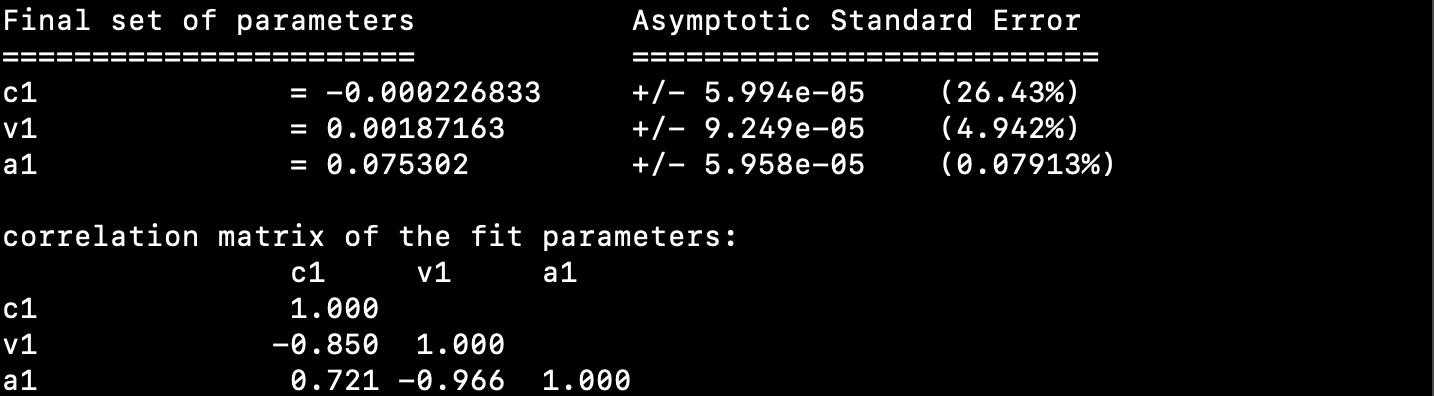
\includegraphics[scale=0.55]{assets/gnuplot_shots/21.png}
    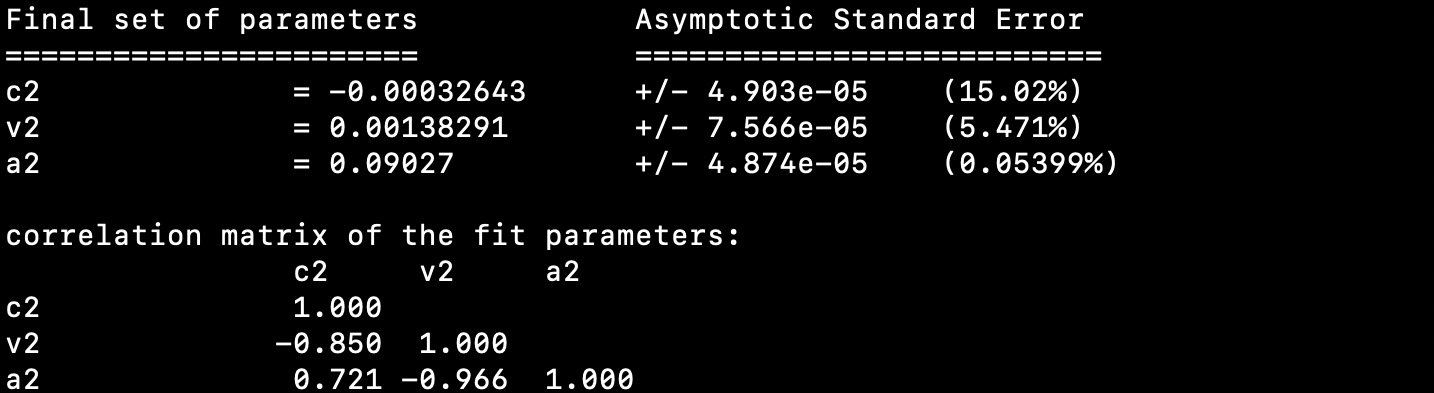
\includegraphics[scale=0.55]{assets/gnuplot_shots/22.png}
    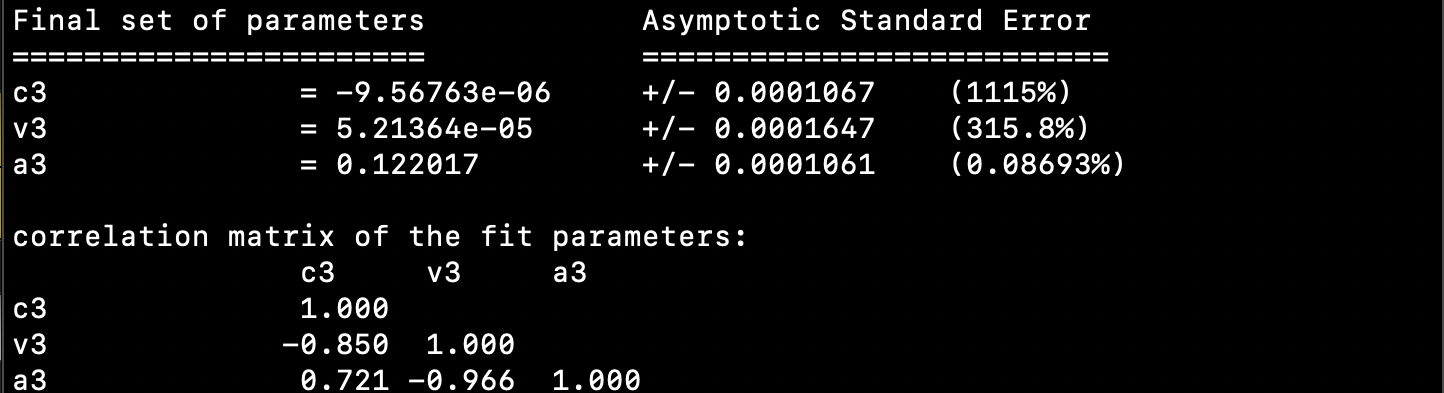
\includegraphics[scale=0.55]{assets/gnuplot_shots/23.png}
    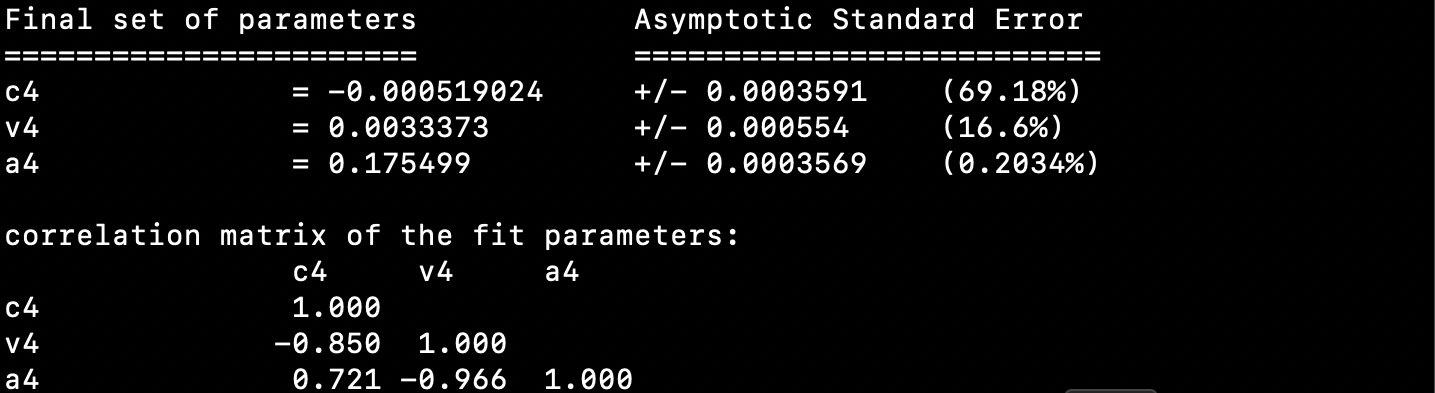
\includegraphics[scale=0.55]{assets/gnuplot_shots/24.png}
    \caption{\texttt{GNUPlot} outputs for the fitting}
    \label{fig:fig8}
\end{figure}
Now we plot the corresponding velocity \(v\) and acceleration \(a\) against \(t\) shown in Figure \ref{fig:fig9} and \ref{fig:fig10}.

We then collect the acceleration values from Figure \ref{fig:fig7} and \ref{fig:fig8} and do a plot of total mass \(M + m\) against the inverse of the acceleration \(a^{-1}\). Then we linearly fit it with a line, whose slope is expected to denote the total net force on the system \(F\) shown in Figure \ref{fig:fig11}\footnote{\textbf{Please Turn Over.}}.
\begin{figure}[H]
    \centering
    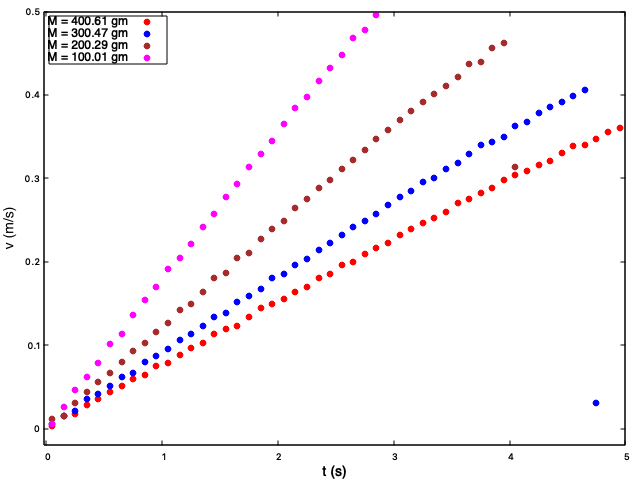
\includegraphics[scale=0.60]{assets/vt_fixed_force.png}
    \caption{Velocity \(v\) against Time \(t\)}
    \label{fig:fig9}
\end{figure}
\begin{figure}[H]
    \centering
    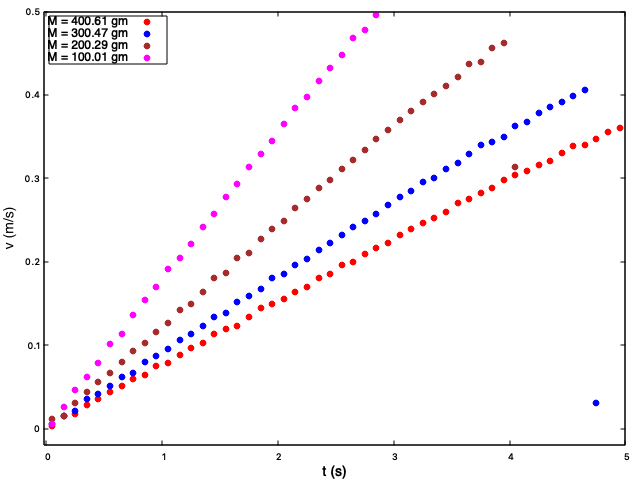
\includegraphics[scale=0.60]{assets/vt_fixed_force.png}
    \caption{Acceleration \(a\) against Time \(t\)}
    \label{fig:fig10}
\end{figure}
\newpage
\begin{figure}[H]
    \centering
    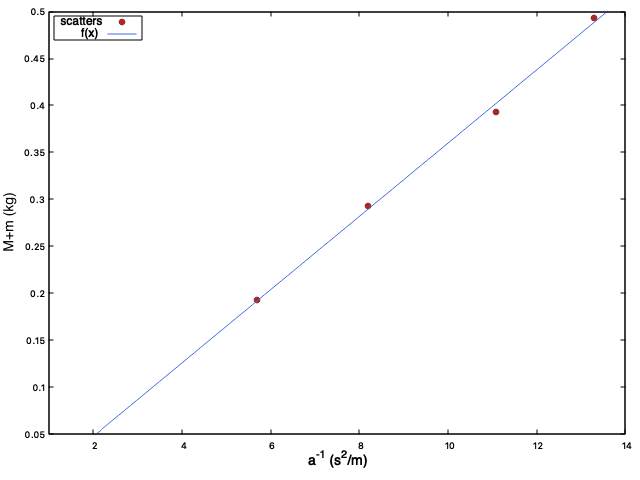
\includegraphics[scale=0.65]{assets/fixedforce_fit.png}
    \caption{The linear fit of total mass \(M + m\) against acceleration \(a\)}
    \label{fig:fig11}
\end{figure}
\begin{algorithm}
    We assume the function of regression to be \[f(x) = mx + c\] where \(f(x)\) denotes the total mass \(M + m\) and \(x\) being the inverse of the acceleration \(a^{-1}\).
\end{algorithm}
\begin{figure}[H]
    \centering
    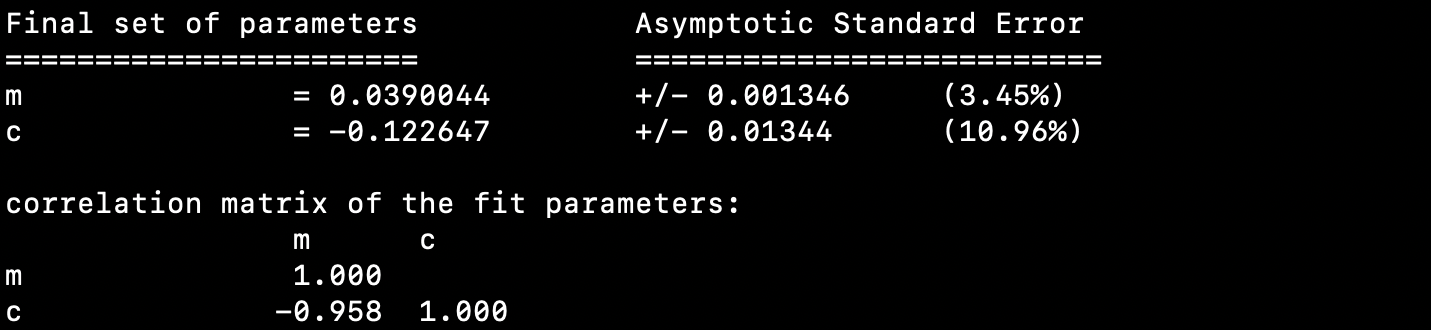
\includegraphics[scale=0.55]{assets/gnuplot_shots/fit2.png}
    \caption{\texttt{GNUPlot} window for the linear regression of \(M+m\) vs. \(a^{-1}\)}
\end{figure}

\newpage

\section{Observation}
\subsection{Case I: Fixed Total Mass}
From the graphs, we can observe that the x vs. t is kind of parabolic. And v vs. t looks linear and a vs. t as line with slope 0, which are all as expected. Also, The value of mass that we got from the slope of Graph of Force vs Fitted Acceleration is 0.112696 kg.

\subsection{Case II: Fixed Net Force}
From the graphs, we can observe that the x vs. t is kind of parabolic. And v vs. t looks linear and a vs. t as line with slope 0, which are all as expected. Also, The value of Force that we get from the slope of Graph of Total Mass vs Inverse Acceleration is 0.0390044 N. 

\section{Error Analysis}
\subsection{Case I: Fixed Total Mass}
The accepted mass of the total fixed mass is equal to (92.52 + 4.13) gm = 96.65 gm = 0.09665 kg. The value of mass that we got from the slope of Graph of Force vs Fitted Acceleration is 0.112696 kg. Thus, the error = 0.016046 kg \\
Hence, percentage error equals = $(0.016046)/(0.09665) * 100 \approx 16.60\%$.

\subsection{Case II: Fixed Net Force}
The accepted value of the fixed force is equal to \(mg = 0.040474\) N. The value of Force that we get from the slope of Graph of Total Mass vs Inverse Acceleration is 0.0390044 N. Thus, error = 0.0014696 N. Hence, the percentage error equals = $(0.0014696/0.040474) * 100 \approx 3.63 \%$.

\section{Conclusion}
We succesfully ended up to show that Newton's 2nd Law is valid, i.e., \[F = ma\] and \[m = F/a\] by those linear curves with pretty small error. Although, we hope we will minimize the errors in upcoming experiments.

\section{Acknowledgements}
\textsc{Thanks} to the instructors and the TAs for such basic but beautiful experiment.
\end{document}